\section{Flujo de trabajo}
\label{ch:propuesta:sec:flujoDeTrabajo}

Actualmente existen flujos de trabajo para la extracción de supeficies \cite{Ruprecht94ascheme}\cite{Dietrich_marchingcubes}, los cuales intentan generar superficies sin los principales problemas topológicos explicados en \ref{subsec:marchingCubes:consecuencias}. El flujo de trabajo propuesto en esta investigación se muestra en la fugura \ref{f:flujoDeTrabajo:flujoDeTrabajo}

\begin{figure}[htb]
\centering
	\includegraphics[width=0.5\textwidth]{images/misc/workflow.pdf}
\caption{Flujo de trabajo propuesto}
\label{f:flujoDeTrabajo:flujoDeTrabajo}
\end{figure}

Cada uno de estos pasos serán explicados a continuación.
\newpage

\subsection{Extracción de datos}
\label{ch:propuesta:sec:extraccionDeDatos}

En primera instancia, para extraer una superficie desde una nube de puntos, es necesario recolectar estos puntos, para eso existen diversas técnicas y propósitos. Para el propósito de esta investigación, el formato de los datos debe ser un \emph{dataset} de imágenes coaxiales que individualmente muestran una sección planar de la superficie que se quiere extraer, y en conjunto describen la superficie completa.

\subsubsection{Imágenes por resonancia magnética}
\label{ch:propuesta:sec:extraccionDeDatos:subsec:imagenesPorResonanciaMagnetica}

En el análisis de imágenes médicas, en ocaciones se necesita visualizar \emph{datasets} volumétricos, cortes en tres dimensiones de los órganos que se quieren estudiar, como las imágenes obtenidas por resonancia magnética (\emph{MRI}, de sus siglas en inglés \emph{Magnetic resonance imaging}).

Las imágenes por resonancia magnética son una técnica de imagenología usada principalmente en el área médica para producir imágenes de alta calidad del interior del cuerpo humano. Estas imágenes son basadas en el principio de la resonancia nuclear magnética, una técnica espectroscópica usada por científicos para obtener información física y química acerca de las moléculas. Ya en el año 2003 existían aproximadamente más de diez mil unidades de resonancia magnética y aproximadamente setenta y cinco millones de exámenes realizados por año \footnote{Joseph P. Hornak, Ph.D. \textit{The Basics of MRI}, http://www.cis.rit.edu/htbooks/mri/ (19 sept. 2012).}

Las imágenes obtenidas de estos exámenes pueden ser pensadas como imágenes en tres dimensiones donde cada \emph{pixel} (o \emph{voxel}, elemento de volúmen) representa una cantidad medible de volumen en alguna posición $(x, y, z)$ del espacio. Un ejemplo de estas imágenes se muestra en la figura \ref{f:flujoDeTrabajo:mri_joe} \footnote{MRI, CPO Abdomen Total, paciente Joe Cabezas Campos, estudio 040501000, Integramedica, Av. Libertador Bernardo O'Higgins 1620, 26 junio 2012 19:35}

\begin{figure}[p]
\centering
	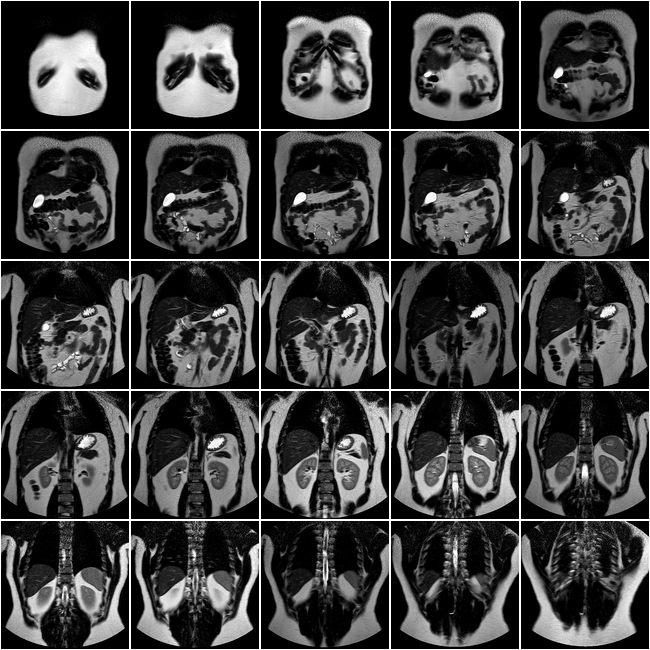
\includegraphics[width=1.0\textwidth]{images/misc/mri_joe.png}
\caption{Un \emph{dataset} de 28 imágenes de un examen de resonancia magnética}
\label{f:flujoDeTrabajo:mri_joe}
\end{figure}

Una forma de visualizar el cuerpo en tres dimensiones es extrayendo una \emph{isosuperficie} usando el algoritmo de \emph{Marching Cubes}.

En esta investigación, la totalidad de los dataset usados para la implementación del algoritmo de \emph{Marching Cubes} son extraidos de imágenes de resonancia magnética.
\newpage

\subsubsection{Funciones en tres dimensiones}
\label{ch:propuesta:sec:extraccionDeDatos:subsec:funcionesEnTresDimensiones}

Otra forma de obtener puntos en un espacio es usando una función matemática de tres dimensiones que asocie cualquier punto de un espacio a un valor escalar. El algoritmo de \emph{Marching Cubes} hace uso de una discretización del espacio ya que cada vértice de cada cubo está apoyado en un punto discreto del espacio, debido a la continuidad de una función de tres dimensiones, es posible escoger cualquier tamaño para los cubos, lo que hace posible escoger la resolución que se desee y con ello tener un malla en tres dimensiones más detallada como se explica en \ref{subsec:marchingCubes:consecuencias}, pero necesariamente con más triángulos lo que puede no ser óptimo.

Si se desea extraer la superficie descrita por una función continua en tres dimensiones, para esta investigación es necesario generar las imágenes de las curvas de nivel que finalmente cumplirán la misma función que las imágenes por resonancia magnética. Un ejemplo de una función continua es la ecuación\ref{ecuacionContinua}

\begin{equation}
f(x,y) = \frac{ \sin{(\sqrt{x^2+y^2})} }{ \sqrt{x^2+y^2} }
\label{ecuacionContinua}
\end{equation}

y sus respectivos gráficos y curvas de nivel se muestra en la figura \ref{c:flujo:greaficoDeLaEcuacion}

\begin{figure}[h]

	\begin{subfigure}[b]{0.45\textwidth}
		\centering
		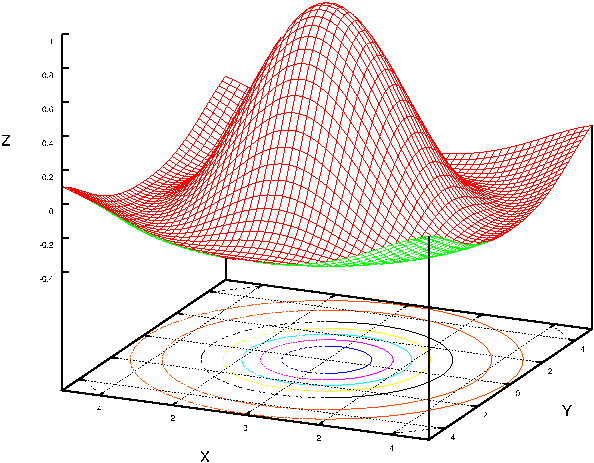
\includegraphics[width=\textwidth]{images/misc/contour_1_using_eps2eps.pdf}
		\caption{Superficie en tres dimensiones}
		\label{c:flujo:superficieEnTresDimensiones}
	\end{subfigure}
	~~
	\begin{subfigure}[b]{0.45\textwidth}
		\centering
		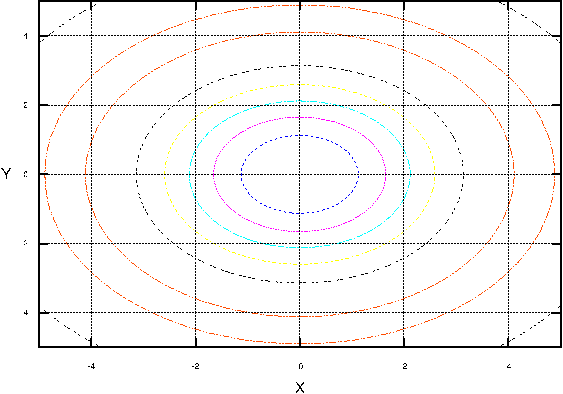
\includegraphics[width=\textwidth]{images/misc/contour_2_using_eps2eps.pdf}
		\caption{Gráfico de curvas de nivel}
		\label{c:flujo:graficoDeCurvasDeNivel}
	\end{subfigure}

	\caption{Gráfico de la ecuación \ref{ecuacionContinua}}
	\label{c:flujo:greaficoDeLaEcuacion}

\end{figure}

Finalmente, cada una de las lineas de las curvas de nivel mostradas en \ref{c:flujo:graficoDeCurvasDeNivel}, representa una imagen de entrada para el algoritmo.

\subsection{Conversión de imágenes}
\label{ch:propuesta:sec:conversionDeImagenes}

Como se plantea en la sección anterior (\ref{ch:propuesta:sec:extraccionDeDatos}), existen varias formas de extraer los datos, por lo que, dependiendo la técnica usada es posible que las imágenes de entrada vengan en diversos formatos también, como se explicará más adelante en \ref{ch:implementacion:sec:datosDeEntrada:subsec:formatodelasimagenesdeentrada}.

Es por esto que, para garantizar una independencia de la implementación hecha en esta investigación con el formato de las imágenes de entrada, se necesita un paso que unifique las diversas formas de extracción de datos para que puedan ser usadas en esta implementación.
Los detalles de la implementación de esto se verá en el capítulo \ref{ch:implementacion}.

Una vez que se asegure que las imágenes de entrada usan el mismo formato, la implementación puede utilizar esta información previa para trabajar haciendo uso de solamente un formato en común, haciendo la implementación más simple. El formato escogido es el formato PGM (\emph{Portable GreyMap}), detalles de su utilización se verán en la sección \ref{ch:implementacion:sec:formatounicoescogido}.

\subsection{Selección del isovalor}
\label{ch:propuesta:sec:seleccionDelIsovalor}

Una vez que se tienen las imágenes de entradas, es momento de escoger una constante que definirá aquellos \emph{pixeles} que estarán dentro o fuera de la superficie que se desea extraer en cada imágen, por lo tanto, la superficie está determinada por este valor llamado \jcq{isovalor}.

Este paso no es trivial, ya que requiere retroalimentación de la superficie extraída, pues en el caso de las imágenes médicas de resonancia magnética, la elección del isovalor puede marcar la diferencia entre ver un cuerpo al nivel del cráneo o al nivel de los huesos internos de éste como se muestra en la figura \ref{c:flujo:superficieDeUnaCalaveraADistintosNivelesDeIsovalor} donde se observa que al aumentar el valor porcentual del isovalor, hay cada vez menos puntos en el espacio que sean menores al isovalor, entregando cada vez una superficie es distinta. La correcta elección del isovalor en las imágenes determina finalmente el nivel de la superficie que se quiere extraer, por ejemplo, si se escoge un valor cero, significa que todos los pixeles quedarán fuera y por lo tanto ningún cubo en el proceso de extracción de superficie tendrá algún vértice marcado como interno, luego, no se generará ningún triángulo y se creará una superficie nula.
Lo mismo ocurre si se escoge un isovalor que sea igual al máximo valor posible en las imágenes.


\begin{figure}[h]

	\begin{subfigure}[b]{0.30\textwidth}
		\centering
		\fbox{
			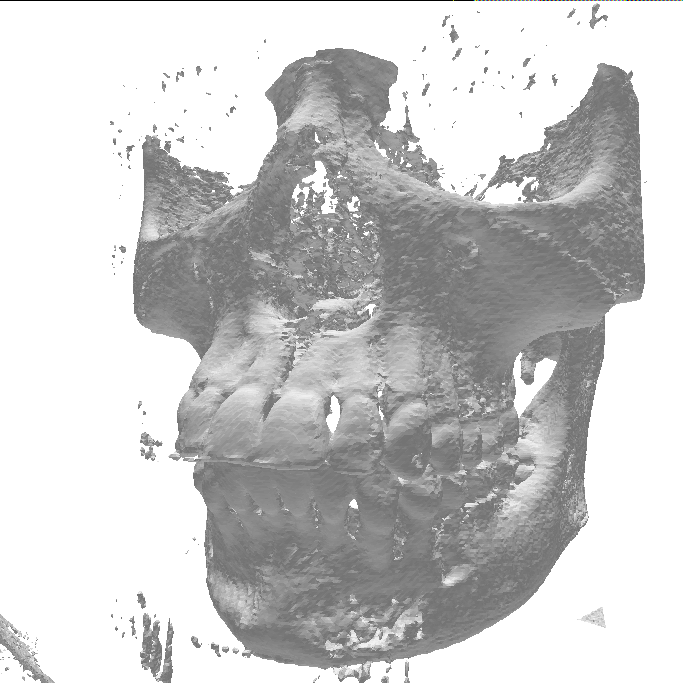
\includegraphics[width=\textwidth]{images/flujo/isovalue/screenshot_15.png}
		}
		\caption{Isovalor de 15\%}
	\end{subfigure}
	\quad
	\begin{subfigure}[b]{0.30\textwidth}
		\centering
		\fbox{
			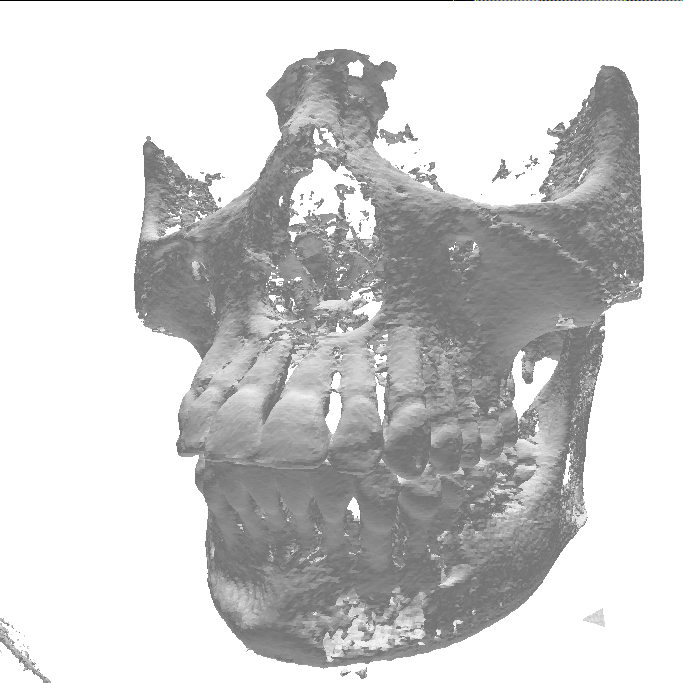
\includegraphics[width=\textwidth]{images/flujo/isovalue/screenshot_20.png}
		}
		\caption{Isovalor de 20\%}
	\end{subfigure}
	\quad
	\begin{subfigure}[b]{0.30\textwidth}
		\centering
		\fbox{
			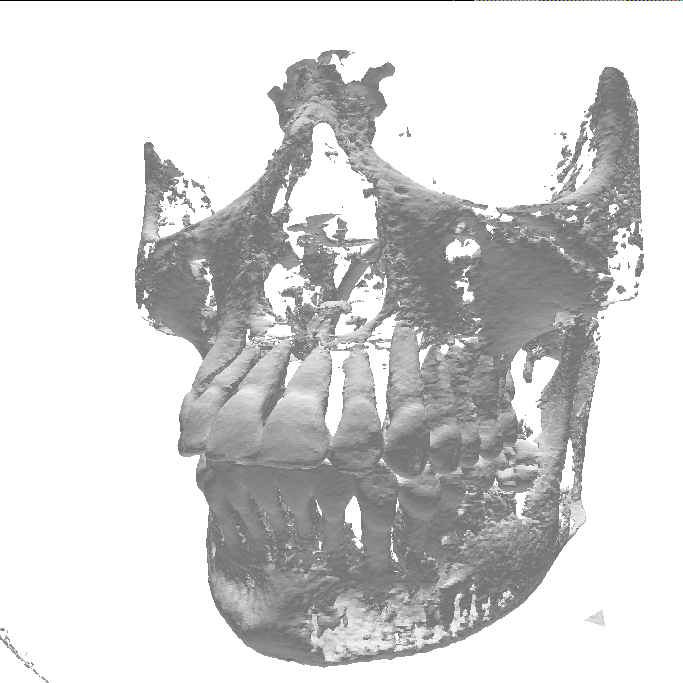
\includegraphics[width=\textwidth]{images/flujo/isovalue/screenshot_25.png}
		}
		\caption{Isovalor de 25\%}
	\end{subfigure}


	\begin{subfigure}[b]{0.30\textwidth}
		\centering
		\fbox{
			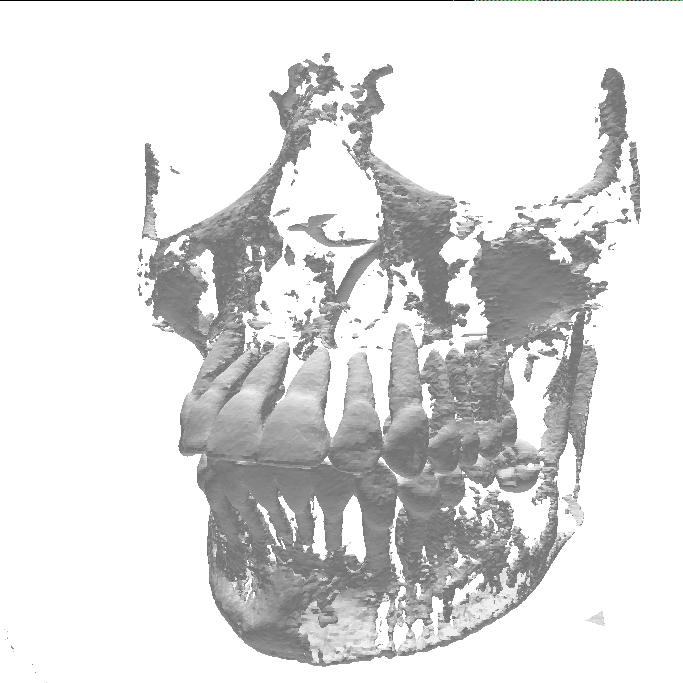
\includegraphics[width=\textwidth]{images/flujo/isovalue/screenshot_30.png}
		}
		\caption{Isovalor de 30\%}
	\end{subfigure}
	\quad
	\begin{subfigure}[b]{0.30\textwidth}
		\centering
		\fbox{
			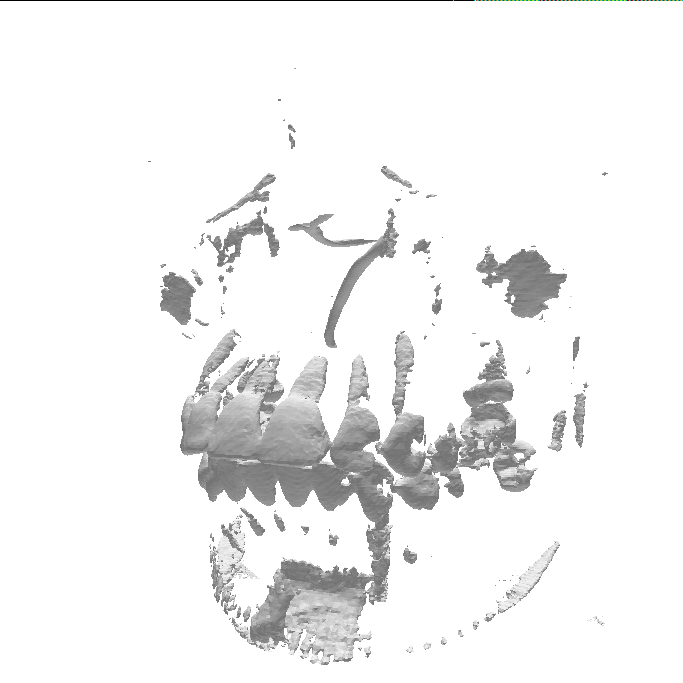
\includegraphics[width=\textwidth]{images/flujo/isovalue/screenshot_40.png}
		}
		\caption{Isovalor de 40\%}
	\end{subfigure}
	\quad
	\begin{subfigure}[b]{0.30\textwidth}
		\centering
		\fbox{
			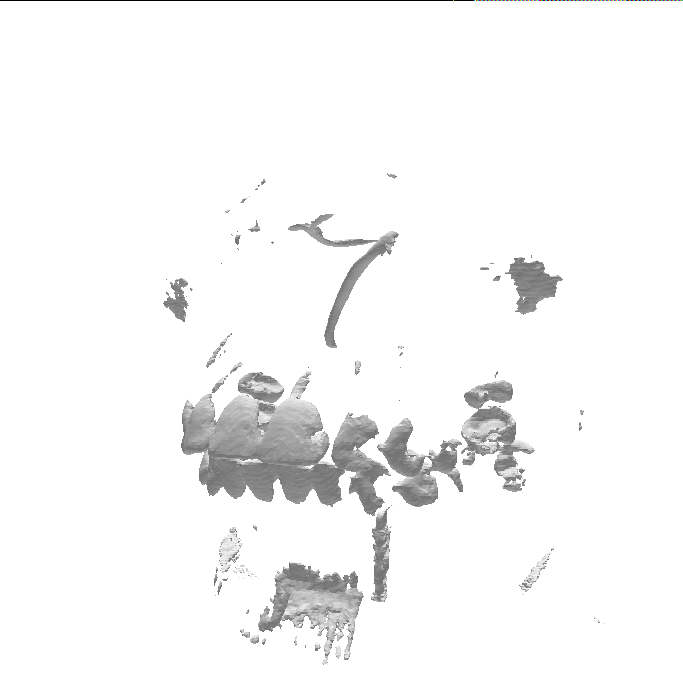
\includegraphics[width=\textwidth]{images/flujo/isovalue/screenshot_45.png}
		}
		\caption{Isovalor de 45\%}
	\end{subfigure}


	% \begin{subfigure}[b]{0.30\textwidth}
	% 	\centering
	% 	\fbox{
	% 		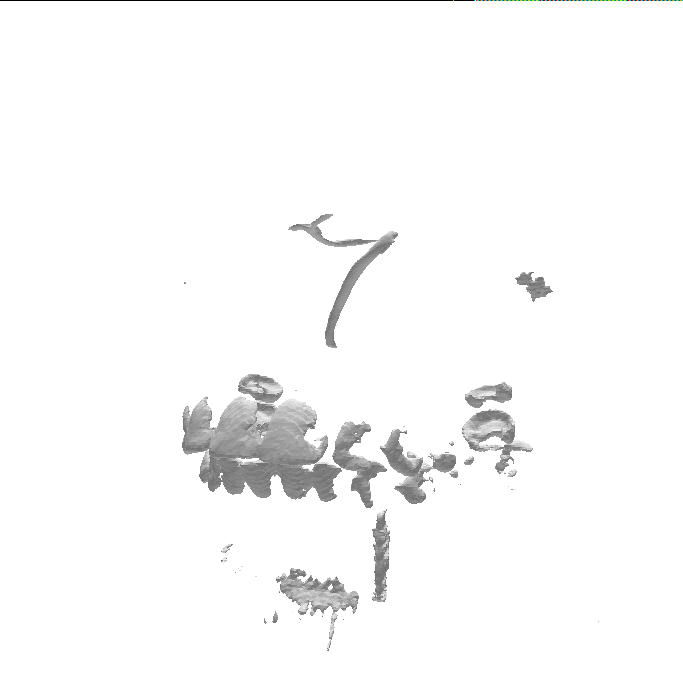
\includegraphics[width=\textwidth]{images/flujo/isovalue/screenshot_50.png}
	% 	}
	% 	\caption{Isovalor de 50\%}
	% \end{subfigure}
	% \quad
	% \begin{subfigure}[b]{0.30\textwidth}
	% 	\centering
	% 	\fbox{
	% 		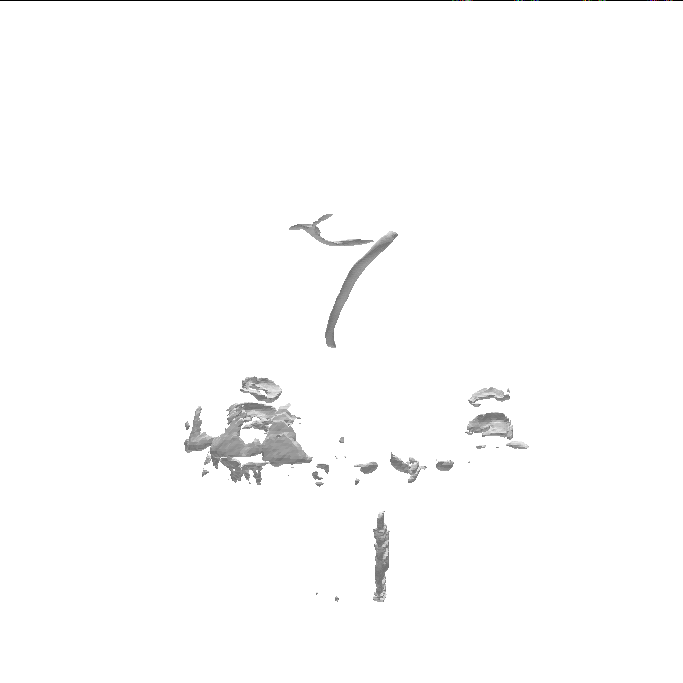
\includegraphics[width=\textwidth]{images/flujo/isovalue/screenshot_60.png}
	% 	}
	% 	\caption{Isovalor de 60\%}
	% \end{subfigure}
	% \quad
	% \begin{subfigure}[b]{0.30\textwidth}
	% 	\centering
	% 	\fbox{
	% 		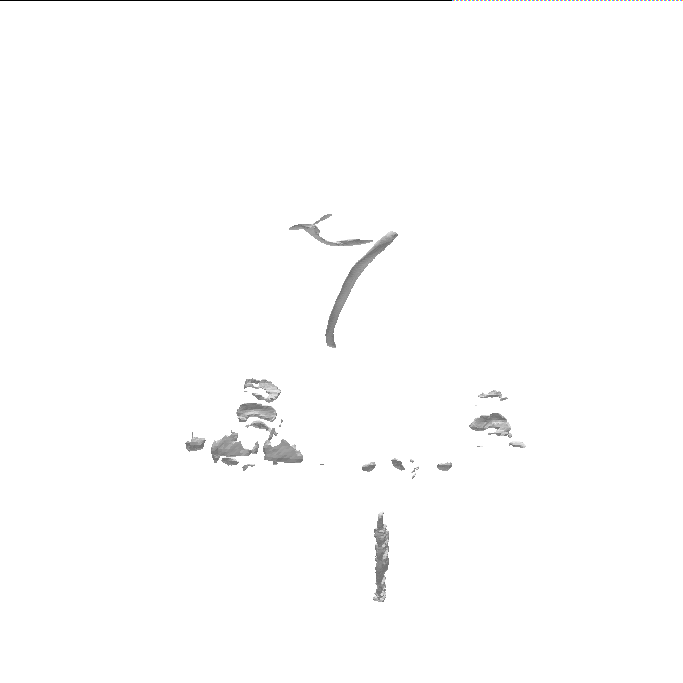
\includegraphics[width=\textwidth]{images/flujo/isovalue/screenshot_65.png}
	% 	}
	% 	\caption{Isovalor de 65\%}
	% \end{subfigure}

	\caption{Superficie de una calavera a distintos niveles de isovalor}
	\label{c:flujo:superficieDeUnaCalaveraADistintosNivelesDeIsovalor}

\end{figure}

En esta implementación, con el fin de garantizar una independencia de las imágenes de entrada con la manipulación del isovalor, el valor del isovalor se escoge porcentualmente, es decir, $0\%$ siginifica que el isovalor vale cero, y una elección de $100\%$ significa que el isovalor vale el máximo valor posible. Esto es porque dependiendo del nivel de profundidad de color de las imágenes, estas pueden ser expresadas entre 0--255 valores (8 bits) y 0--65536 valores (16 bits).

\subsection{Extracción de la superficie}
\label{ch:propuesta:sec:extraccionDeLaSuperficie}

Luego de escoger el isovalor adecuado, el siguiente paso es extraer la superficie usando el isovalor, por esto se le llama \jcq{isosuperficie}.

Esta investigación tiene su mayor enfoque en este punto ya que es en este paso donde se utiliza el algoritmo de \emph{Marching Cubes} para la extracción. Se desarrolló un \emph{software} que genera la superficie usando un isovalor porcentual ajustable por el usuario, y permite visualizar y navegar en tres dimensiones el modelo generado, una imagen del programa desarrollado se muestra en la figura \ref{f:flujoDeTrabajo:visualizer_1}. La principal característica de este visualizador es que es posible editar el isovalor y ver el cambio de la isosuperficie en tiempo real, permitiendo de esta manera corregir el isovalor usado para obtener el nivel de isovalor apropiado.

\begin{figure}[h]
\centering
	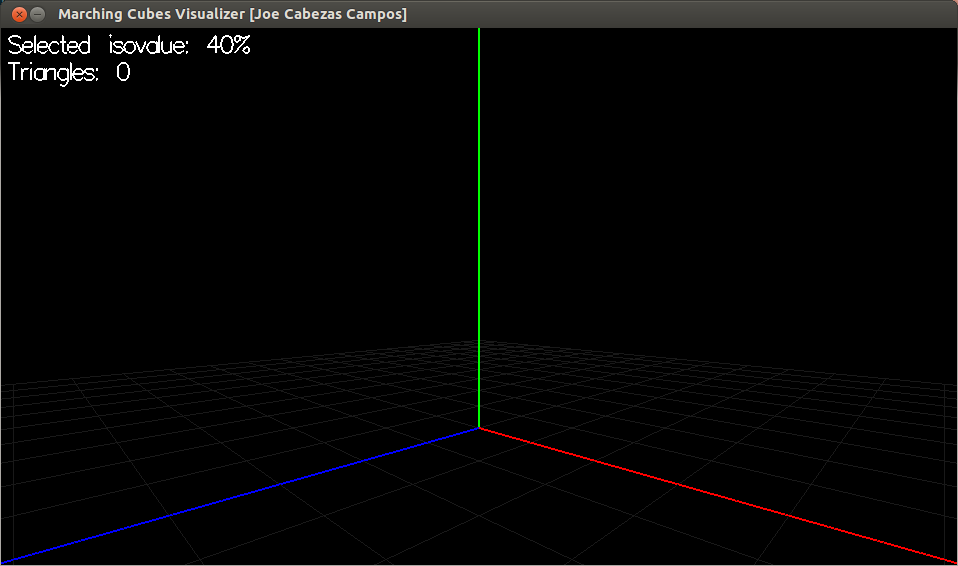
\includegraphics[width=1.0\textwidth]{images/visualizer/visualizer_1.png}
\caption{Programa visualizador de superficies generadas usando \emph{Marching Cubes}}
\label{f:flujoDeTrabajo:visualizer_1}
\end{figure}

\subsubsection{Ejecución}
\label{ch:propuesta:sec:extraccionDeLaSuperficie:subsec:ejecucion}

El programa recibe como parámetros de entrada una lista de las imágenes ordenadas que se desean usar como \emph{dataset}, de la siguiente manera:

\begin{quote}
./MemoriaJoeCabezasCode \textbf{[archivo1.pgm] [archivo2.pgm] [...]}
\end{quote}

Debido a que los \emph{dataset} normalmente están conformados por cientos de imágenes, se hace uso de la flexibilidad de los programas que vienen en el núcleo de Linux, en primer lugar el comando \textbf{\emph{ls}} lista el contenido de un directorio\footnote{http://manpages.ubuntu.com/manpages/precise/en/man1/ls.1.html (20 sept. 1012)}, y si se agrega la opcion \textbf{\emph{-1}} lista un archivo por linea, por lo que es más fácil revisar si están en orden los archivos, los cuales deberían venir en orden alfabético.

Un ejemplo de un listado de archivos es el siguiente:

\begin{verbatim}
joe@joe-ultrabook:pgm $ ls -1
out00000.pgm
out00001.pgm
out00002.pgm
out00003.pgm
out00004.pgm
out00005.pgm
out00006.pgm
out00007.pgm
out00008.pgm
out00009.pgm
\end{verbatim}

en el ejemplo anterior, se listaron los únicos 10 archivos dentro de un directorio \jcq{pgm/}, luego, esta salida puede usarse como entrada del programa que necesita la lista de archivos, la forma de hacer esto es usando el operador \textbf{\emph{\$()}}, el cual evalúa lo que está dentro del paréntesis y devuelve el resultado, como se muestra a continuación:

\begin{verbatim}
./MemoriaJoeCabezasCode $(ls -1 pgm/*)
\end{verbatim}

Lo que es equivalente a hacer:

\begin{verbatim}
./MemoriaJoeCabezasCode out00000.pgm \
out00001.pgm \
out00002.pgm \
out00003.pgm \
out00004.pgm \
out00005.pgm \
out00006.pgm \
out00007.pgm \
out00008.pgm \
out00009.pgm
\end{verbatim}

Finalmente el programa es ejecutado con éxito e inmediatamente se presenta la ventana principal como se muestra en la figura \ref{f:flujoDeTrabajo:visualizer_1}

\subsubsection{Interfaz}
\label{ch:propuesta:sec:extraccionDeLaSuperficie:subsec:interfaz}

La interfaz es simple, el programa muestra en su completitud una ventana OpenGL\footnote{http://www.opengl.org/} y en la esquina superior izquierda un panel de estado que indica el isovalor actual (porcentual) y la cantidad de triángulos de la superficie, como se muestra en la figura \ref{f:flujoDeTrabajo:interface}

\begin{figure}[h]
\centering
	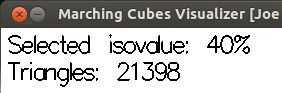
\includegraphics[width=0.5\textwidth]{images/visualizer/interface.png}
\caption{Panel de estado, con un isovalor del 40\%, se crea una superficie que esta formada por $172416$ triángulos.}
\label{f:flujoDeTrabajo:interface}
\end{figure}

\subsubsection{Modo de uso}
\label{ch:propuesta:sec:extraccionDeLaSuperficie:subsec:modoDeUso}

Es posible usar el programa tanto con teclado como con un control de Xbox360\textsuperscript{\textregistered}\footnote{http://www.microsoft.com/hardware/en-us/p/xbox-360-controller-for-windows (20 sept. 2012)}.

El programa además puede capturar imágenes en formato \emph{PNG} (Portable Network \mbox{Graphics}\footnote{http://www.libpng.org/pub/png/}), generando imágenes con nombre cuyo formato es:

\begin{quote}
	screenshot\_\textbf{\textless isovalor porcentual\textgreater}.png
\end{quote}

También es posible exportar la superficie que se está visualizando a un archivo de modelo 3D (archivo \emph{OFF}), para así poder ser importado en otro programa que acepte este formato como geomview\footnote{http://www.geomview.org/}, como se muestra en la figura \ref{f:flujoDeTrabajo:geomview}

\begin{figure}[!htb]
\centering
	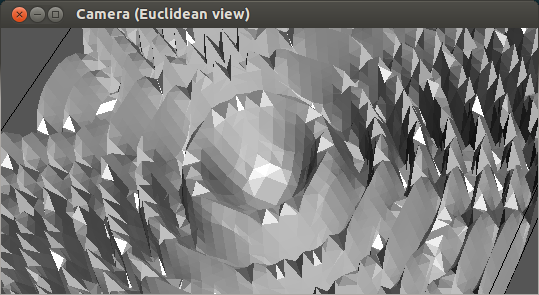
\includegraphics[width=0.7\textwidth]{images/visualizer/geomview.png}
\caption{Superficie generada en el visualizador, importada como archivo OFF en \mbox{geomview}}
\label{f:flujoDeTrabajo:geomview}
\end{figure}

\newpage
En un principio, el progama no muestra ninguna superficie, ya que esta debe ser generada presionando \keystroke{ENTER} o 
\includegraphics[scale=0.4, trim= 0 20 0 0]{images/visualizer/xbox360/start.png}. Por defecto el isovalor porcentual usado es de un $40\%$, pero puede ser modificado usando la tecla \keystroke{F1} o 
\includegraphics[scale=0.4, trim= 0 20 0 0]{images/visualizer/xbox360/leftShoulder0.png} para disminuir el valor del isovalor y la tecla \keystroke{F2} o 
\includegraphics[scale=0.4, trim= 0 20 0 0]{images/visualizer/xbox360/rightShoulder0.png} para aumentar el isovalor. El valor del isovalor seleccionado se puede ver en el panel de informacion como se muestra en la figura \ref{f:flujoDeTrabajo:interface}.

Dependiendo de la complejidad, cantidad y resolución de las imágenes de entrada y del isovalor usado para generar la superficie, es posible que la supeficie esté compuesta por cientos de miles de triángulos lo que puede ralentizar el sistema y hacer difícil la navegación, es por esto que en cualquier momento, el modelo puede ser eliminado para poder así vaciar memoria y hacer la navegación mas fácil, esto sólo afecta a la superficie, los ejes y el plano cartesiano guía siempre son visibles. Para poder eliminar la superficie se debe presionar la tecla \keystroke{Backspace} o 
\includegraphics[scale=0.4, trim= 0 20 0 0]{images/visualizer/xbox360/select.png}.

A continuación se muestra una tabla con las teclas de control\footnote{Imágenes obtenidas desde https://github.com/sgraham/gamepad.js/ (20 sept. 2012)}\footnote{Xbox 360 Icon Pack por Jeff Jenkins, @sinnix, http://sinnix.net/downloads/?did=1 (20 sept. 2012)}:

\begin{longtable}[c]{
	|>{\centering}m{3.0cm}<{\centering}|
	m{3cm}||
	l|
}
\hline
Teclado & Control Xbox360 & Acción \\ \hline
	\huge{\keystroke{\large{W}}} &
	
\includegraphics[scale=0.4]{images/visualizer/xbox360/leftStick.png} (arriba) &
	Avanzar
	\\ \hline

	\huge{\keystroke{\large{A}}} &
	
\includegraphics[scale=0.4]{images/visualizer/xbox360/leftStick.png} (izquierda) &
	Desplazarse hacia la izquierda
	\\ \hline

	\huge{\keystroke{\large{S}}} &
	
\includegraphics[scale=0.4]{images/visualizer/xbox360/leftStick.png} (derecha) &
	Retroceder
	\\ \hline

	\huge{\keystroke{\large{D}}} &
	
\includegraphics[scale=0.4]{images/visualizer/xbox360/leftStick.png} (abajo) &
	Desplazarse hacia la derecha
	\\ \hline

	\huge{\keystroke{\large{$\downarrow$}}} &
	\centering 
\includegraphics[scale=0.4]{images/visualizer/xbox360/leftShoulder1.png} &
	Descender
	\\ \hline

	\huge{\keystroke{\large{$\uparrow$}}} &
	\centering 
\includegraphics[scale=0.4]{images/visualizer/xbox360/rightShoulder1.png} &
	Ascender
	\\ \hline

	\huge{\keystroke{\large{$\leftarrow$}}} &
	
\includegraphics[scale=0.4]{images/visualizer/xbox360/rightStick.png} (izquierda) &
	Girar hacia la izquierda
	\\ \hline

	\huge{\keystroke{\large{$\rightarrow$}}} &
	
\includegraphics[scale=0.4]{images/visualizer/xbox360/rightStick.png} (derecha) &
	Girar hacia la derecha
	\\ \hline

	\huge{\keystroke{\large{F1}}} \normalsize{o} \huge{\keystroke{\large{-}}} &
	\centering 
\includegraphics[scale=0.6]{images/visualizer/xbox360/leftShoulder0.png} &
	Disminuir el isovalor
	\\ \hline

	\huge{\keystroke{\large{F2}}} \normalsize{o} \huge{\keystroke{\large{+}}} &
	\centering 
\includegraphics[scale=0.6]{images/visualizer/xbox360/rightShoulder0.png} &
	Aumentar el isovalor
	\\ \hline

	\huge{\keystroke{\large{Enter}}} &
	\centering 
\includegraphics[scale=0.6]{images/visualizer/xbox360/start.png} &
	Generar isosuperficie (\emph{Marching Cubes})
	\\ \hline

	\huge{\keystroke{\large{Backspace}}} &
	\centering 
\includegraphics[scale=0.6]{images/visualizer/xbox360/select.png} &
	Destruye isosuperficie
	\\ \hline

	\huge{\keystroke{\large{R}}} &
	\centering 
\includegraphics[scale=0.6]{images/visualizer/xbox360/dpadLeft.png} &
	Rotar superficie en eje X (horario)
	\\ \hline

	\huge{\keystroke{\large{F}}} &
	\centering 
\includegraphics[scale=0.6]{images/visualizer/xbox360/dpadRight.png} &
	Rotar superficie en eje X (antihorario)
	\\ \hline

	\huge{\keystroke{\large{T}}} &
	\centering 
\includegraphics[scale=0.6]{images/visualizer/xbox360/dpadUp.png} &
	Rotar superficie en eje Y (horario)
	\\ \hline

	\huge{\keystroke{\large{G}}} &
	\centering 
\includegraphics[scale=0.6]{images/visualizer/xbox360/dpadDown.png} &
	Rotar superficie en eje Y (antihorario)
	\\ \hline

	\huge{\keystroke{\large{P}}} &
	\centering 
\includegraphics[scale=0.6]{images/visualizer/xbox360/faceButton0.png} &
	Capturar imagen (\emph{screenshot})
	\\ \hline

	\huge{\keystroke{\large{O}}} &
	\centering 
\includegraphics[scale=0.6]{images/visualizer/xbox360/faceButton1.png} &
	Exportar modelo 3D (archivo \emph{OFF})
	\\ \hline

	\huge{\keystroke{\large{F11}}} &
	\centering 
\includegraphics[scale=0.6]{images/visualizer/xbox360/faceButton2.png} &
	Alternar modo pantalla completa
	\\ \hline

	\huge{\keystroke{\large{Esc}}} &
	\centering 
\includegraphics[scale=0.6]{images/visualizer/xbox360/faceButton3.png} &
	Salir
	\\ \hline

\end{longtable}

\subsubsection{Navegación}
\label{ch:propuesta:sec:extraccionDeLaSuperficie:subsec:navegacion}

En un principio el programa muestra el sistema de coordenadas cartesianas, los ejes $X$, $Y$ y $Z$ son mostrados como lineas de color rojo, verde y azul respectivamente, junto a un plano cartesiano sujeto al plano $X-Z$, en $Y=0$ formado por una grilla de lineas grises. Esto sirve como guía al desplazarse en el espacio para así no perder de vista el punto de origen.

La navegación implementada ocupa un esquema en tercera persona en la cual el desplazamiento con las teclas de movimiento (\keystroke{W}, \keystroke{A}, \keystroke{S} y \keystroke{D} o 
\includegraphics[scale=0.4, trim= 0 20 0 0]{images/visualizer/xbox360/leftStick.png}) mueve la cámara en el plano $XZ$, mientras que para girar la cámara se usa lan teclas de giro de cámara (\keystroke{$\leftarrow$} y \keystroke{$\rightarrow$} o 
\includegraphics[scale=0.4, trim= 0 20 0 0]{images/visualizer/xbox360/rightStick.png}). Sin embargo, si se una un control de Xbox360\textsuperscript{\textregistered} el mando 
\includegraphics[scale=0.4, trim= 0 20 0 0]{images/visualizer/xbox360/rightStick.png} además de controlar el giro en el eje $Y$, controla el acimut\footnote{Ver glosario.} de la cámara, por lo tanto es posible también mirar hacia arriba y hacia abajo, moviendo el mando hacia arriba y hacia abajo respectivamente.

Para controlar la elevación (posicion en el eje $Y$) se usan las teclas de elevación (\keystroke{$\uparrow$} y \keystroke{$\downarrow$} o 
\includegraphics[scale=0.4, trim= 0 20 0 0]{images/visualizer/xbox360/leftShoulder1.png} y 
\includegraphics[scale=0.4, trim= 0 20 0 0]{images/visualizer/xbox360/rightShoulder1.png}).

Finalmente, con este esquema es posible navegar de una forma homóloga a como lo haría una persona paseando en un museo y con la capacidad de elevarse del suelo, lo cual permite volar al rededor de un objeto sin dejar de mirarlo, por ejemplo, para rodear un objeto girando en en forma radial en sentido horario en una circunferencia en el plano $XY$ se debe presionar \keystroke{A} o 
\includegraphics[scale=0.4, trim= 0 20 0 0]{images/visualizer/xbox360/leftStick.png} (hacia la izquierda) para desplazarse hacia la izquierda mientras se presiona \keystroke{$\rightarrow$} o 
\includegraphics[scale=0.4, trim= 0 20 0 0]{images/visualizer/xbox360/rightStick.png} (hacia la derecha). De la misma forma, se puede girar en sentido anti-horario presionando \keystroke{D} o 
\includegraphics[scale=0.4, trim= 0 20 0 0]{images/visualizer/xbox360/leftStick.png} (hacia la derecha) para desplazarse hacia la derecha mientras se presiona \keystroke{$\leftarrow$} o 
\includegraphics[scale=0.4, trim= 0 20 0 0]{images/visualizer/xbox360/rightStick.png} (hacia la izquierda).

\subsubsection{Características especiales}
\label{ch:propuesta:sec:extraccionDeLaSuperficie:subsec:caracteristicasEspeciales}

El programa visualizador además permite capturar imágenes (conocidas como \emph{screenshots}) y exportar la superficie generada con el isovalor seleccionado como un modelo de tres dimensiones en un archivo \emph{OFF} como se explico en la seccion \ref{ch:propuesta:sec:extraccionDeLaSuperficie:subsec:modoDeUso}, para capturar una imagen se debe presionar la tecla \keystroke{P} o 
\includegraphics[scale=0.4, trim= 0 20 0 0]{images/visualizer/xbox360/faceButton0.png} y para guardar la superficie como un archivo \emph{OFF} se debe presionar la tecla \keystroke{O} o \includegraphics[scale=0.4, trim= 0 20 0 0]{images/visualizer/xbox360/faceButton1.png}.

Es posible ocupar el visualizador ocupando toda la pantalla simplemente alternando el \jcq{Modo pantalla completa}, el que por defecto esta desactivado en un comienzo, para alternar al modo pantalla completa se debe presionar la tecla \keystroke{F11} o \includegraphics[scale=0.4, trim= 0 20 0 0]{images/visualizer/xbox360/faceButton2.png}, el efecto de esto se muestra en la figura \ref{c:flujo:alternandoModoPantallaCompleta}.

\begin{figure}[htbp]

	\begin{subfigure}[b]{\textwidth}
		\centering
		\includegraphics[width=0.6\textwidth]{images/visualizer/visualizer_fullscreen_0.png}
		\caption{Modo pantalla completa desactivado}
		\label{c:flujo:visualizer_fullscreen_0}
	\end{subfigure}
	%~

	\begin{subfigure}[b]{\textwidth}
		\centering
		\includegraphics[width=0.6\textwidth]{images/visualizer/visualizer_fullscreen_1.png}
		\caption{Modo pantalla completa activado}
		\label{c:flujo:visualizer_fullscreen_1}
	\end{subfigure}

	\caption{Alternando modo pantalla completa}
	\label{c:flujo:alternandoModoPantallaCompleta}

\end{figure}

\subsection{Refinamiento}
\label{ch:propuesta:sec:refinamiento}

Luego de extraer la superficie usando un isovalor adecuado es momento de refinar la superficie generada con el fin de mejorar su calidad, hacerla mas liviana disminuyendo la cantidad de triángulos y reparando los problemas causados por el algoritmo de \emph{Marching Cubes} que se explicaron en la seccion \ref{subsec:marchingCubes:consecuencias}.

Para esto se ocupará una herramienta externa llamada \emph{CGAL}\footnote{http://www.cgal.org/ (20 sept 2012)} (\emph{The Computational Geometry Algorithms Library}). \emph{CGAL} es una librería en \emph{C++} que provee un acceso fácil, eficiente y eficaz a una colección de algoritmos geométricos. La librería \emph{CGAL} es usada en diversas áreas de la computación geométrica como diseño asistido por computadora, gráficos de computadora, visualización científica (como en este caso), modelamiento, sistemas geográficos, biología molecular, etc.

Esta librería ofrece estructuras de datos y algoritmos como triangulaciones, polígonos, poliedros, generación de mallas, procesamiento geométrico (que es lo que se pretende hacer en este paso del flujo), etc.

\subsection{Reconstrucción de superficie}
\label{ch:propuesta:sec:refinamiento:reconstruccionDeSuperficie}

\emph{CGAL} provee un método de reconstrucción de superficies que toma como entrada una colección de puntos en el espacio con sus respectivas normales orientadas y calcula una función implícita\footnote{http://www.cgal.org/Manual/latest/doc\_html/cgal\_manual/Surface\_reconstruction\_points\_3/Chapter\_main.html (20 sept. 2012)}. \emph{CGAL} asume que los puntos de entrada no contienen puntos atípicos y vienen con algo de ruido.

La superficie generada se calcula extrayendo una isosuperficie de esta función calculada anteriormente usando un generador de mallas de superficies \cite{Rineau2007100} o potencialmente con cualquier otro algoritmo de extracción de superficies. La función calculada es un función aproximada del sólido inferido (\emph{Poisson Surface Reconstruction}). \emph{Poisson} es un proceso de dos pasos, primero necesita resolver la ecuación implícita, y luego evaluar esta función.

\subsection{Poisson}
\label{ch:propuesta:sec:refinamiento:poisson}

Dado un set de puntos en tres dimensiones con normales orientadas, en primer lugar, el método \emph{Poisson Surface Reconstruction} \cite{Kazhdan2006PoissonSurfaceReconstruction} resuelve una función aproximada del sólido que mejor se adapte a las gradientes de las normales de los puntos de entrada, luego a esa función se le extrae una isosuperficie usando una versión adaptativa de \emph{Marching Cubes} llamada \emph{Adaptative Marching Cubes} \cite{Shu95adaptivemarching}

% \subsection{Ejemplo}
% \label{ch:propuesta:sec:refinamiento:ejemplos}

Un ejemplo que muestra la nube de puntos de entrada y la superficie generada en \emph{CGAL} usando el método \emph{Poisson Surface Reconstruction}, se muestra en la figura \ref{c:flujo:poissonSurfaceReconstruction}

\begin{figure}[h]

	\begin{subfigure}[b]{0.45\textwidth}
		\centering
			\includegraphics[width=\textwidth]{images/flujo/refinamiento_1_0.jpg}
			\caption{$17000$ puntos de entrada con normales orientadas}
			\label{f:flujoDeTrabajo:refinamiento_1_0}
	\end{subfigure}
	~
	\begin{subfigure}[b]{0.45\textwidth}
		\includegraphics[width=\textwidth]{images/flujo/refinamiento_1_1.jpg}
		\caption{La superficie reconstruida usando el algoritmo}
		\label{f:flujoDeTrabajo:refinamiento_1_1}
	\end{subfigure}

	\caption{\emph{Poisson Surface Reconstruction}}
	\label{c:flujo:poissonSurfaceReconstruction}

\end{figure}

%TODO
%obtener imagenes de http://www-sop.inria.fr/members/Pierre.Alliez/demos/sm/slides.pdf

% Además es posible hacer ajustes previos a la reconstrucción que modifican la superficie obtenida bajo parámetros como el ángulo mínimo de los triángulos, radio máximo de los triángulos (determina el tamaño de éstos), ajustes...

\subsection{Exportación}
\label{ch:propuesta:sec:exportacion}

Finalmente, en este paso, ya se tiene la malla de superficie deseada gracias al proceso de selección (\ref{ch:propuesta:sec:seleccionDelIsovalor}) y extracción de la superficie (\ref{ch:propuesta:sec:extraccionDeLaSuperficie}) y refinada gracias al paso de refinamiento (\ref{ch:propuesta:sec:refinamiento}). El último paso ahora es exportar el modelo en tres dimensiones a un formato útil para el proposito que fue extraído, que puede ser para modelamiento, visualizacion y otros propósitos ya mencionados en la sección \ref{sec:usosDeLasMallasGeometricas}